Durante el desarrollo, se ha tenido en cuenta que la aplicación tiene que ser fácil de usar por el usuario. Si bien es un prototipo sencillo, siempre es necesaria una explicación sobre el uso básico del mismo. En este pequeño manual, vamos a ver cómo utilizar el prototipo desarrollado, así como mostrar ejemplos de uso del mismo.  Mostraremos primero los tipos de ventana disponibles, y después se explicará la colección de acciones que puede realizar el usuario.\\

\begin{figure}[H]
\begin{center}

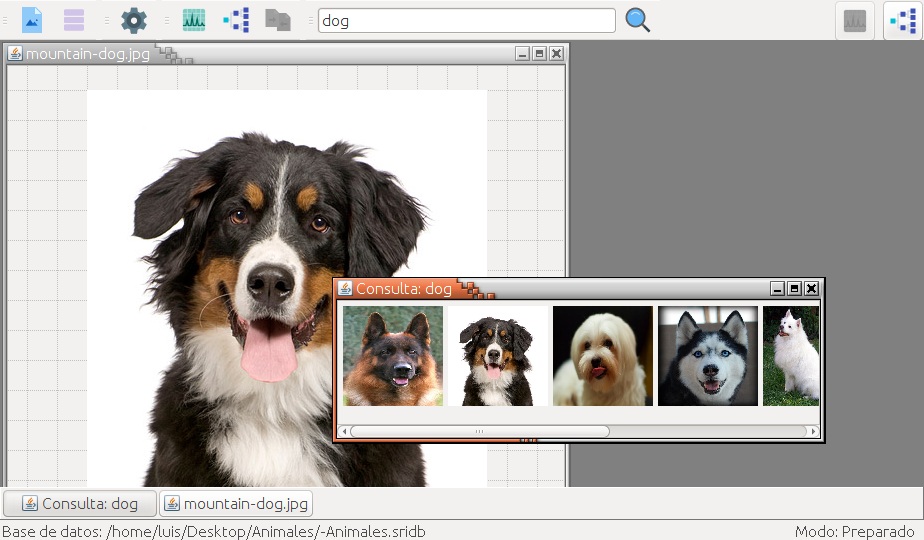
\includegraphics[width=0.9\textwidth]{img/v-uso.png}
\end{center}

\caption{Aplicación en uso.}
\end{figure}

\newpage
\section{Ventana principal}

\begin{figure}[H]
\begin{center}

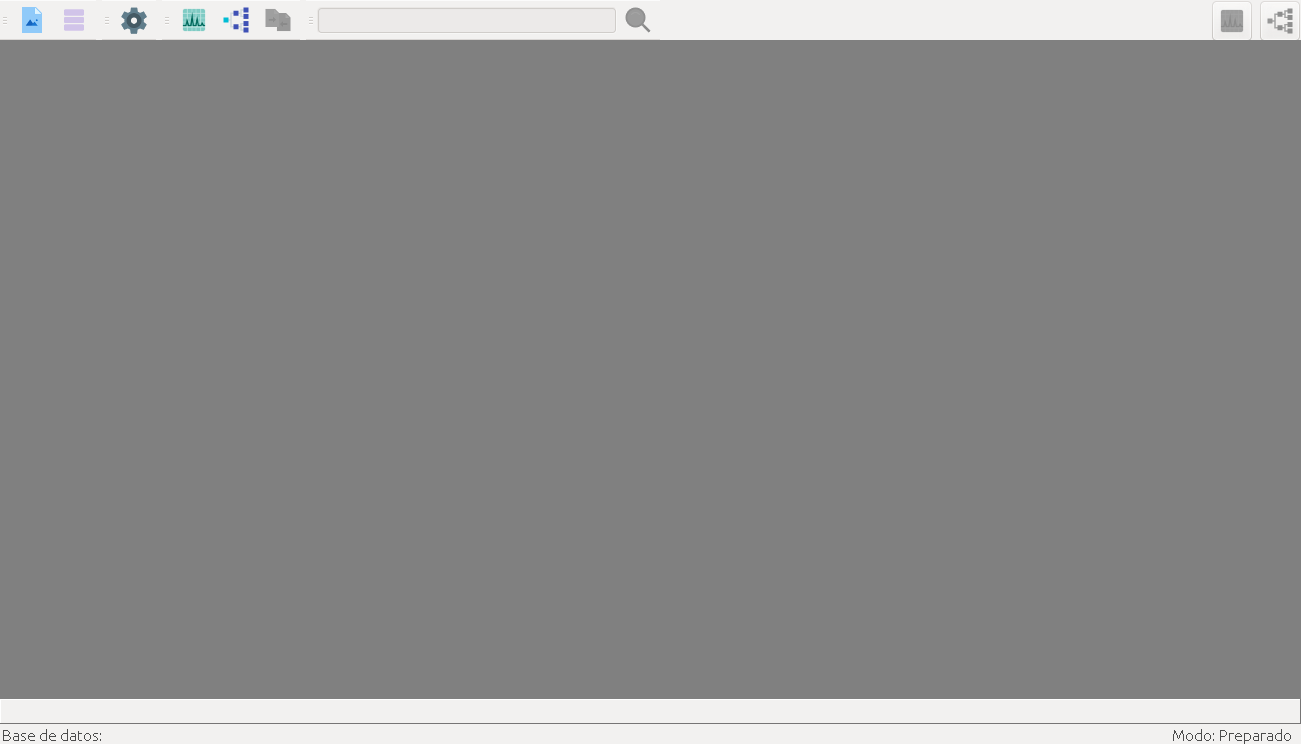
\includegraphics[width=0.9\textwidth]{img/v-principal.png}
\end{center}

\caption{Ventana principal.}
\end{figure}

La ventana principal es el centro de la aplicación. Permite acceder de manera rápida al usuario a todas las herramientas de la aplicación. Cuenta con un escritorio donde manejar las demás ventanas de la aplicación, junto con una barra para poder gestionar las ventanas abiertas y una barra de estado, que muestra información de la base de datos abierta y el estado actual de la aplicación, preparado para realizar más acciones o ocupado calculando algún resultado.\\

Además, dependiendo del tipo de base de datos activa unas funcionalidades y deja bloqueadas otras, indicándolo mediante el color de los propios botones (en color si están activos y en blanco y negro si están inactivos) así como con dos iconos en la parte superior izquierda que sirven para marcar el tipo de base de datos activa.

En la sección \ref{acciones} se puede encontrar un listado completo de las acciones vinculadas a los botones de esta pantalla que puede realizar el usuario.\\

\newpage
 
\section{Ventana de imagen}
\begin{figure}[H]
\begin{center}

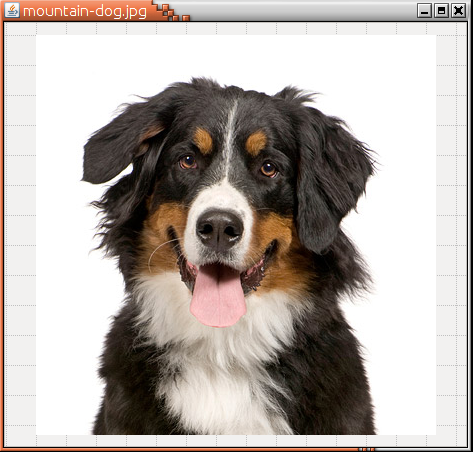
\includegraphics[width=0.9\textwidth]{img/v-imagen.png}
\end{center}

\caption{Ventana imagen.}
\end{figure}

Ventana donde se muestra una imagen. Teniendo activada una ventana interna de este tipo, se puede calcular el descriptor adecuado para cada tipo de entrada. Es decir, se puede calcular la clasificación de una imagen natural y también  se puede calcular el descriptor de una forma.\\



\newpage
\section{Ventana de clasificación}
\begin{figure}[H]
\begin{center}

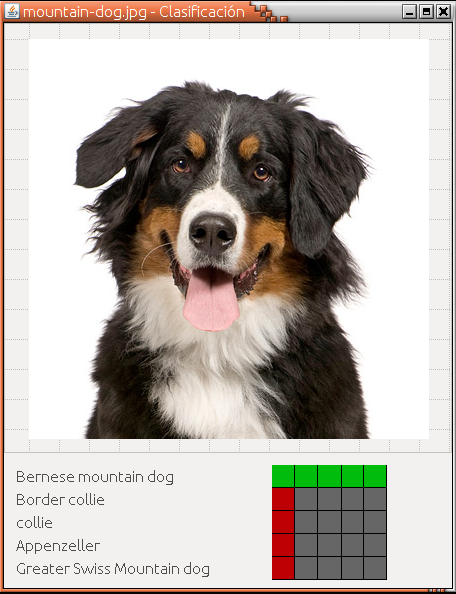
\includegraphics[width=0.9\textwidth]{img/v-clasificacion.png}
\end{center}

\caption{Ventana de clasificación.}
\end{figure}

Se muestra la imagen clasificada, así como las cinco clases con mejor valoración. A la derecha de esos nombres se muestra una representación gráfica de dichos valores. Hay cinco posibles valoraciones, siendo la mejor valoración posible cinco cuadrados verdes y la peor un solo cuadrado rojo.\\
 

\newpage
\section{Ventana de descriptor}
\begin{figure}[H]
\begin{center}

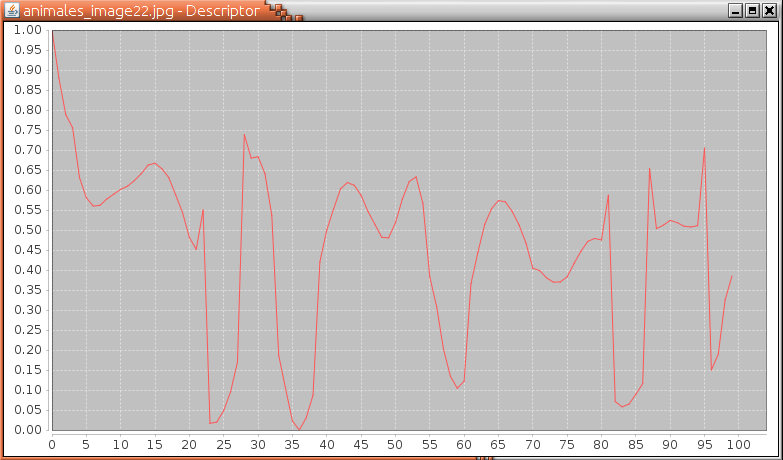
\includegraphics[width=1\textwidth]{img/v-descriptor.png}
\end{center}

\caption{Ventana de descriptor.}
\end{figure}


Esta ventana interna muestra el descriptor de una forma. El descriptor se muestra en forma de gráfica, la forma más natural de representar la información que contiene.

\newpage
\section{Ventana de resultados de búsqueda}
\begin{figure}[H]
\begin{center}

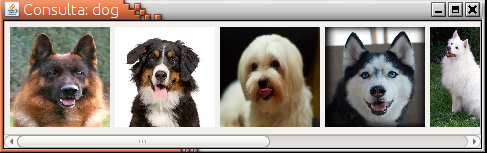
\includegraphics[width=0.9\textwidth]{img/v-resultado.png}
\end{center}

\caption{Ventana de resultados.}
\end{figure}

Esta ventana contiene los resultados de una búsqueda. Se ordenan de izquierda a derecha, según el grado de cumplimiento de la consulta. Se puede colocar el cursor para conocer el valor de acierto de la búsqueda para cada una de las imágenes, así como desplazarse entre la lista usando la barra de desplazamiento.\\

El valor de acierto de la búsqueda empieza en 0, que representa el acierto absoluto, y según se aleje del mismo peor será su cumplimiento. En el caso de búsqueda por conceptos, el peor valor es un 1, mientras que en la búsqueda por formas, el peor valor es 100.\\



\newpage
\section{Acciones}
\label{acciones}

\begin{figure}[H]
\begin{center}

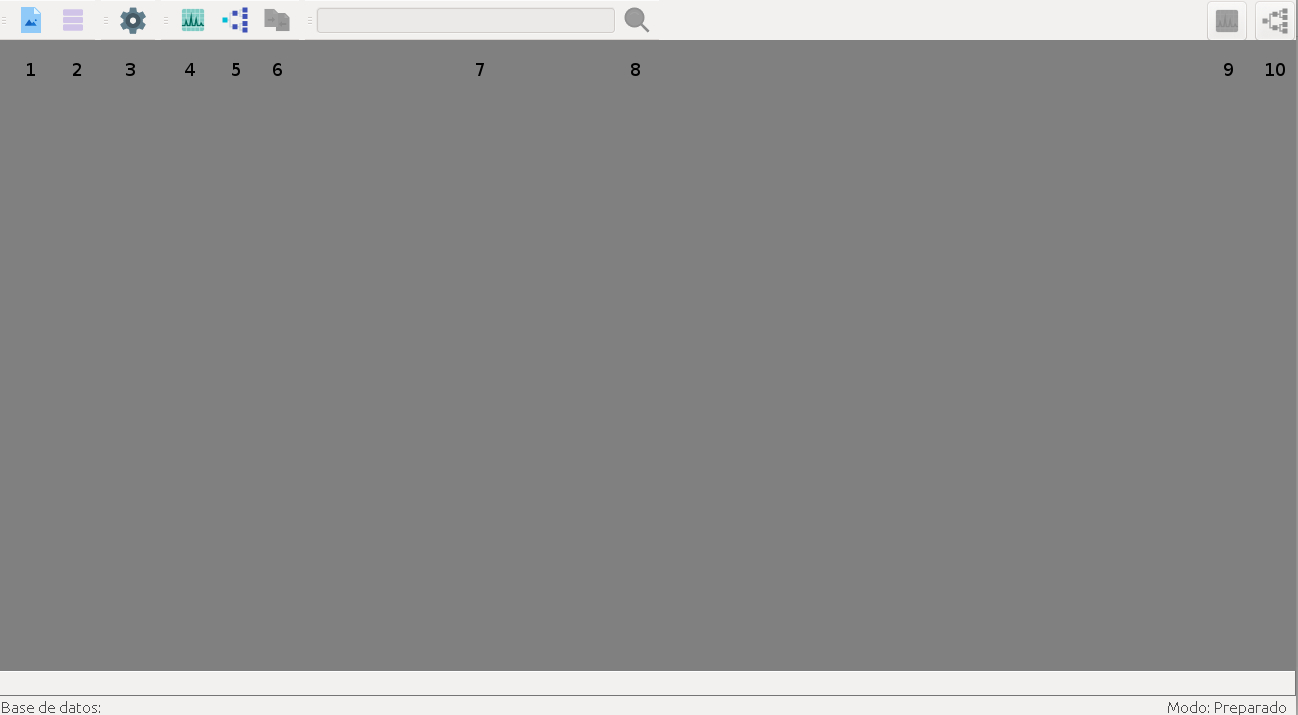
\includegraphics[width=0.9\textwidth]{img/v-principal-enum.png}
\end{center}

\caption{Ventana principal enumerada.}
\end{figure}
Vamos a describir las acciones que puede realizar el usuario:
\begin{itemize}
\item \textbf{Abrir imagen: }Para abrir una imagen, primero se clica sobre el botón ``Abrir imagen''(1). Aparecerá un menú donde se deberá seleccionar la imagen deseada. Tras esto se obtendrá como resultado una ventana con la imagen seleccionada.
\item \textbf{Abrir base de datos:}Para abrir una base de datos, primero se clica sobre el botón de ``Abrir base de datos'' (2). Aparecerá un menú donde se deberá seleccionar la base de datos deseada. Tras esto, se cargará la base de datos en la aplicación, indicándose así en la barra de estado.
\item \textbf{Calcular descriptor: } Teniendo una imagen activa. El usuario clica sobre el botón  ``Cálculo de descriptor''(4) y obtiene como resultado la ventana de dicho descriptor. El usuario puede hacer click derecho sobre el botón ``Cálculo de descriptor''(4) para cambiar el tipo de descriptor a calcular.
\item \textbf{Calcular clasificación: } Teniendo una imagen activa.  El usuario clica sobre el botón  ``Cálculo de clasificación''(5) y obtiene como resultado la ventana de clasificación asociada.
\item \textbf{Comparar descriptor con la base de datos: } Con una base de datos de tipo ``descriptor'' activa y una ventada de descriptor seleccionada, se clica en el botón de ``comparar''(6). Tras esto, el usuario obtendrá una ventana con los resultados de la búsqueda.
\item \textbf{Buscar un concepto en la base de datos: } Con una base de datos de tipo ``clasificación'' activa, se introduce en el campo de texto(7) la palabra a buscar y se clica en el ``botón de búsqueda''(8) o se presiona la tecla ENTER. Tras esto, se le mostrará al usuario una ventana con los resultados de su búsqueda.
\end{itemize}